\documentclass[a4paper]{article}

%% Language and font encodings
\usepackage[english]{babel}
\selectlanguage{english}
\usepackage[utf8x]{inputenc}
\usepackage[T1]{fontenc}
\usepackage{graphicx}

%% Sets page size and margins
\usepackage[a4paper,top=3cm,bottom=2cm,left=3cm,right=3cm,marginparwidth=1.75cm]{geometry}

%% Useful packages
\usepackage{amsmath}
\usepackage[sc]{mathpazo}
\usepackage{graphicx}
\usepackage[colorinlistoftodos]{todonotes}
\usepackage[colorlinks=true, allcolors=blue]{hyperref}
\usepackage{amsmath}

\title{Heurísticas y Optimización combinatoria: Soluciones a instancias del Problema del Agente Viajero por medio de Recocido Simulado}
\author{Karla Socorro García Alcántara}

\begin{document}
\maketitle

%\begin{abstract}
%Your abstract.
%\end{abstract}

\section{Introducción}

En este reporte presento la heurística de Recocido Simulado en una versión modificada (Aceptación por Umbrales) para resolver instancias del Problema del Agente Viajero también en una de sus variantes (buscando una trayectoria en vez de un ciclo), conocido por pertenecer a la clase de Problemas NP-Duros. Abordaré brevemente algunos detalles de la implementación y exhibiré los resultados obtenidos.

\section{Problema del Agente Viajero}
Consiste en encontrar un ciclo (debemos empezar y terminar en el mismo punto) que recorra un conjunto de ciudades que necesita recorrer un "agente" de algún negocio; hacer el recorrido de una ciudad a otra tiene un $costo$, por lo que se busca el ciclo que más barato le resulte al agente.
En nuestra versión modificada sólo buscamos una trayectoria que visite todas las ciudades de un cierto conjunto (a esto llamamos $instanci$a) con el menor costo total posible.

\section{Heurística de Recocido Simulado}

Esta heurística de optimización combinatoria se basa en la práctica de recocido de cerámica y metales para mejorar su propiedad de tenacidad, en esta práctica se cuece la pieza que se está forjando o moldeando para posteriormente dejarla enfriar, mientras más lento se enfríe resulta más tenaz.\\ Es utilizada para resolver instancias de problemas NP-Duros, que los algortimos deterministas conocidos no han conseguido resolver o lo han logrado de manera poco satisfactoria; al "resolver" una instancia, el Recocido Simulado entrega la solución más óptima encontrada.
\\
En la variante de Aceptación por Umbrales establecemos nuestro espacio de búsqueda similar a una gráfica en la que cada nodo \textit{n} representa una solución y su nodo vecino \textit{v} es una solución que se parece lo suficiente a \textit{n}; la relación de parecido entre una solución y su vecina cambia para cada implementación de la heurística. Además establecemos una función de costo $\mathcal{F}(s)$ para cuantificar qué tan buena es una solución $s$.
\\
En la heurística modificada establecemos un valor $\varphi$ y un valor $\varepsilon$; trabajará a partir de una solución inicial $s_{1}$, temperatura inicial $t_{1}$, para alcanzar una temperatura final $t-final$. Para llegar a esta temperatura generaremos un lote $LOTE_{i}$ de soluciones a partir de $s_{1}$ aplicando una función $\mathcal{V}(s_{1})$ para encontrar sus vecinas y aceptando únicamente las soluciones $s'$ que cumplan con $\mathcal{F}(s') < \mathcal{F}(s) + t_{1}$; repetimos este procedimiento para generar el lote $LOTE_{i + 1}$ reasignando a $s_{1}$ con el valor de la última solución $s'$ generada en el lote más reciente ($LOTE_{i}$) y disminuimos la temperatura $t$ multiplicándola por $\varphi$ en caso de que la diferencia del promedio del costo de las soluciones entre el $LOTE_{i}$ y el $LOTE_{i - 1}$ sea menor que el valor que hemos establecido como $\varepsilon$.

Partiendo de lo anterior podemos intuir que el valor de $\varphi$ que es un factor para reducir la temperatura del sistema que puede ser sintonizado para acelerar la heurística teniendo como consecuencia soluciones poco optimizadas; y que los demás parámetros sólo se pueden sintonizar para mejoría con experimentación.

\section{Integración Heurística -  Problema}
Para ejemplificar Recocido Simulado sobre el Problema del Agente Viajero tenemos las ciudades que hay que visitar representadas como nodos de una gráfica $E \in G$, cuyas aristas $e \in E$ son la abstracción de rutas de avión entre un par de ciudades $v$ y $u$. Cuando un par de ciudades no están conectadas, le asignamos una distancia $P$ muy alta; en el caso de mi implementación tomamos la distancia máxima entre dos ciudades en $G$ multiplicado por el factor de castigo $C$, el cual asigné como $C = 2$. Recordando que en el Problema del Agente Viajero buscamos la solución de menor costo, tomaremos a la más óptima encontrada por la heurística como la que cubre esta característica.
Se implementaron las siguientes fórmulas preestablecidas:
\begin{itemize}
\item  Función de costo:
\[F(s) = \frac{\sum_{i =2}^{k} w'(v_i , v_{i-1})}{A(|S| - 1)}\]
\item Pares conectados:
\[E_s = \{(u, v): u, v \in S y (u, v) \in E\}\]
\item Promedio de pesos(distancias):
\[A = \frac{\sum_{e \in E_s} w(e)}{|E_s|}\]
\item Factor de castigo:
\[P(S) = f(max\{s\})\]
\item Función de peso aumentado:
\[w' = \begin{cases}
      w(u, v), si (u, v) \in E \\
      {P,      e.o.c} \\

   \end{cases}
\]
\end{itemize}

\section{Experimentación}

Para los experimentos buscamos soluciones óptimas para instancias de 40 y 150 ciudades.
Sintonicé el programa con los siguientes parámetros:
\begin{itemize}
\item $\varphi = 0.9$
\item $\varepsilon = 0.00001$
\item $t_final = 0.0001$
\item $t_1 = 4.0$
\item Tamaño de $LOTE = 500$
\item Distancia asignada a ciudades desconectadas: $max(u, v) * 2, (u, v) \in G$
\item Factor de castigo: $C = 2$
\end{itemize}
Cuando encontramos una nueva solución verificamos si están conectadas consecutivamente, si es así la consideramos como una función factible, en caso contrario es no factible; en la búsqueda de soluciones factibles óptimas, la aceptación por umbrales nos permite escapar de mínimos locales del espacio de búsqueda utilizando una búsqueda similar a $Hill climbing$ y $Gardient descent$.

Para inicializar el programa se utiliza una $semilla$ que utilizará el generador de números aleatorios para mezclar la instancia que deseamos explorar y establecer el inicio de la búsqueda.
Por elemplo, en la experimentación encontré que hay soluciones que se evalúan con una función de costo muy similar, y dan resultados muy similares sin que exista una relación entre los números utilizados, por ejemplo, para 40 ciudades la semilla $600$ arrojó:\\
Costo: 0.6354061393419022, factible: true \\
Ciudades:\\
829,986,505,839,447,345,717,22,216,893,493,935,272,521,492,710,572,113,642,853,137,\\774,1032,74,299,786,627,180,607,1073,109,679,921,747,200,857,498,178,117,830\\
\\
\\
Mientras que la semilla $333$:\\
Costo: 0.6354061391648228, factible: true\\
Ciudades:
830,117,178,498,857,200,747,921,679,109,1073,607,180,627,786,299,74,1032,774,137,\\853,642,113,572,710,492,521,272,935,493,893,216,22,717,345,447,839,505,986,829\\
\\
Para esta instancia, la mejor solución que encontré fue con la semilla $1971$:\\
Costo: 0.6316032582947841, factible: true\\
Ciudades:
829,986,505,839,447,345,717,22,216,935,493,893,521,492,272,710,572,113,642,853,137,\\774,1032,299,74,627,786,180,607,1073,109,921,679,747,200,498,178,857,117,830\\
\\
La gráfica que muestra la evaluación del costo de todas las soluciones encontradas en su ejecución se muestra a continuación.\\
\\
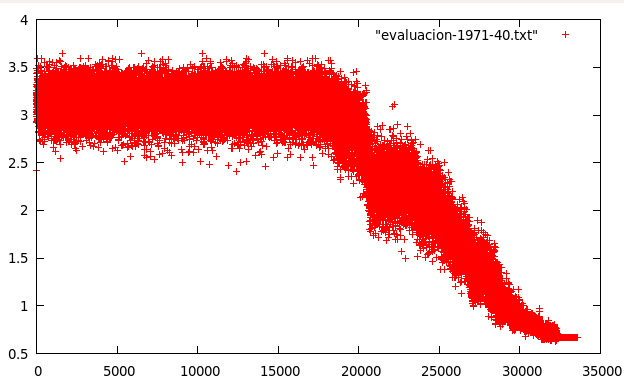
\includegraphics[width=\textwidth]{graficas/grafica-1971-40.png}\\
\\
Para la instancia de 150 ciudades encontré:\\
Semilla: 89754553\\
Costo: 0.28374620645543386, factible: true\\
Ciudades:\\
830,178,39,857,712,865,517,1072,313,700,454,552,955,833,547,94,398,119,302,385,86,74,\\
408,438,297,757,876,697,670,414,853,1080,1034,871,890,741,796,705,323,492,203,489,877,\\
393,563,885,159,254,981,919,271,319,256,991,591,413,957,308,213,717,872,587,332,206,219,\\
654,576,447,355,688,98,1069,477,278,233,639,95,611,986,111,79,281,505,486,358,528,935,\\
837,284,257,893,766,347,1016,614,896,96,735,40,67,470,69,748,795,571,933,190,1007,359,12,\\
675,186,107,151,44,299,115,627,293,637,93,785,607,395,854,10,1002,189,690,156,557,341,1037,\\
234,582,679,535,1057,13,478,243,583,515,410,498,497,669,310,117,337\\
\\
Cuya gráfica de costos es:


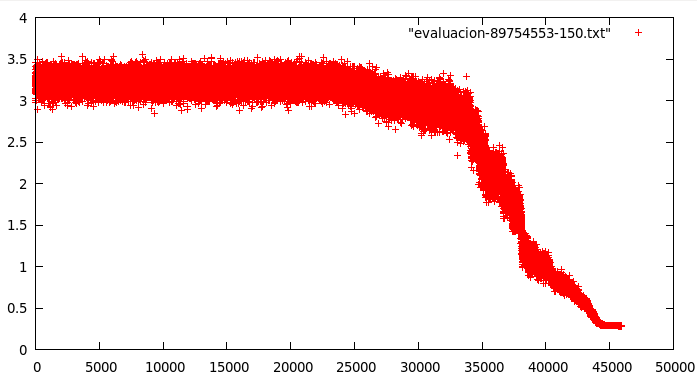
\includegraphics[width=\textwidth]{graficas/grafica-89754553-150.png}\\
\\
\section{Conclusiones}

Con este proyecto comprendemos una forma de abordar instancias reales de problemas NP-Duros, que sólo con experimentación se pueden mejorar los resultados y que no podemos asegurar que hemos encontrado la mejor solución; esto implicaría analizar todas las soluciones del espacio de búsqueda y perderíamos toda optimización. Estos procedimientos resultan útiles para la vida real, ya que la vida real está plagada de problemas NP-Duros que como científicos podemos trabajar para solucionar de manera óptima.



\end{document}
